\documentclass{standalone}
\usepackage{tikz}

\usetikzlibrary{calc}
\usetikzlibrary{through}
\usetikzlibrary{intersections}

\begin{document}

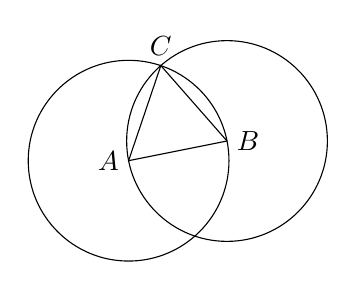
\begin{tikzpicture}
  \coordinate [label=left:$A$]  (A) at ($ (0,0) $);
  \coordinate [label=right:$B$] (B) at ($ (1.25,0.25) $);

  \draw (A) -- (B);

  \node [name path=D, draw, circle through=(B)] at (A) {};
  \node [name path=E, draw, circle through=(A)] at (B) {};

  \path [name intersections={of=D and E,by={[label=above:$C$]C}}];
  \draw (A) -- (C) -- (B);
\end{tikzpicture}

\end{document}
